\documentclass[12pt]{report}

\usepackage{graphicx} % images
\usepackage{tikz} % grafike
\usetikzlibrary{positioning}
\usepackage{forest} % drevo za memo
\usepackage{float}
\usepackage[hidelinks]{hyperref}

% required formating
\usepackage[a4paper, left=2.5cm, right=2.5cm, top=2.5cm, bottom=2.5cm]{geometry} % margines
\usepackage[slovene]{babel} % slovenian localization
\usepackage{newtxtext,newtxmath} % times new roman
\usepackage{setspace}
\onehalfspacing
\setlength{\parskip}{0.5em}
\setlength{\parindent}{1.5em}
\usepackage{titlesec}
\titleformat{\chapter} % remove poglavje before chapter titles
  {\normalfont\Huge\bfseries}
  {\thechapter}{1em}{}
\titlespacing*{\chapter}{left}{before}{after}
\titlespacing*{\chapter}{0pt}{0pt}{20pt}

% centriraj img captione
\usepackage{caption}
\captionsetup{justification=centering}

% charts
\usepackage{pgfplots}
\pgfplotsset{compat=1.18}

% koda
\usepackage{algorithm}
\usepackage{algpseudocode}
\floatname{algorithm}{Algoritem}

\title{Vegova}
\author{Vid Furlan}
\date{February 2026}

\begin{document}

\begin{titlepage}
    \begin{figure}
        \centering
        
\includegraphics[width=1\linewidth]{template/logotip_vegova_leze_brezokvirja.png}
    \end{figure}

    \vspace*{5cm}
    \centering
    {\Huge \textbf{Reševanje igre Domineering}}
    
    \vspace*{0.5cm}
    {\large \textbf{Strokovno poročilo za 4. predmet strokovne mature}}

    \vfill
    {\large
    \raggedright Mentor: Nataša Makarovič 
    \hfill Avtor: Vid Furlan
    }

    \vspace*{1.5cm}
    {\large Ljubljana, april 2026}
    
\end{titlepage}

\setcounter{page}{2}
\newpage

\section*{Povzetek}
To poročilo predstavi razvoj algoritma za iskanje optimalne strategije igranja matematične igre Domineering. K problemu naloga pristopi, kot iskanje po grafu stanj, kjer vozlišča grafa predstavljajo stanja. Na začetku poročilo razloži pravila igre, nato pa se osredotoči na razlago iterativnega izboljševanja algoritma. Pri tem opiše in razloži različne tehnike optimiziranja in njihove učinke. Poročilo se zaključi s preprosto analizo rezultatov pridobljenih med testiranjem.

\textbf{Ključne besede: } Domineering, dizajn algoritmov, grafa stanj, tehnike optimiziranja, analiza rezultatov 

\section*{Abstract}
This report presents the development of an algorithm for finding optimal strategies in the mathematical game Domineering. The problem is approached as a state-space search, where each game configuration is treated as a node in a graph. Initially the report describes the game and its rules, and then moves to iteratively improving the search algorithm. It explores different optimization techniques and their effects. The report concludes with a simple analysis of the results obtained from testing.

\textbf{Keywords: } Domineering, algorithm design, state-space search, optimization techniques, performance analysis

\newpage

\tableofcontents
\newpage

\renewcommand{\listalgorithmname}{Kazalo algoritmov}
\begingroup
\let\clearpage\relax
\listoffigures
\listofalgorithms
\endgroup

\newpage

\chapter{Uvod}

Tema reševanje igre Domineering je bila izbrana, saj se rad ukvarjam z algoritmičnimi problemi. Cilj naloge je razviti algoritem za iskanje optimalne strategije in in zmagovalca pod določenimi pogoji. Pri tem želimo razviti čim bolj učinkovito rešitev, ki bo sposobna rešiti čim večje igralne plošče. 

Naloga vključuje implementacijo osnovnega algoritma ter postopno izboljšavo tega z uporabo različnih optimizacij. Rezultate delovanja bomo analizirali in primerjali različne pristope ter ocenili vpliv posameznih optimizacij.

\chapter{Metodologija}

\section{Pristop}
Problem smo obravnavali kot preiskovanje prostora stanj. Najprej smo implementirali osnovni brute force algoritem, ki preizkusi vse možne poteze. Zaradi eksponentne rasti iskalnega prostora smo pristop postopoma izboljševali z različnimi optimizacijami, na koncu pa razvite algoritme testirali na Arnesovem superračunalniku.

\section{Razvoj}
Najprej smo implementirali osnovni rekurzivni algoritem, nato pa dodali memoizacijo, zmanjšali obiskan del iskalnega prostora in mnoge druge optimizacije. Za lažji razvoj in vizualizacijo smo razvili še dodatna orodja, kot je program za merjenje časa izvajanja programa in vizualizator grafa igre.

\section{Uporabljena orodja in tehnologije}
Algoritmi so bili realizirani v programskem jeziku C++, ostala orodja pa v Pythonu. V C++ smo se izogibali uporabi dodatnih zunanjih knjižnic, kot so Boost, saj je bil cilj čim več algoritmov in podatkovnih struktur implementirati samostojno. V Pythonu pa je bil za vizualizacijo uporabljen Plotly, NetworkX za obdelavo grafov in Qt 6 za izdelavo uporabniških vmesnikov. Projekt je bil razvit v okolju Linux z uporabo orodja CMake, zaradi lažje poznejše integracije z okoljem na superračunalniku.

\section{Testiranje}
Algoritem smo testirali z merjenjem časa izvajanja na različnih velikostih igralnih plošč. Primerjali smo osnovni algoritem z optimiziranimi različicami ter analizirali vpliv posameznih optimizacij.

\chapter{Predstavitev problema}
\section{Pravila igre}
Domineering je strateška igra za dva igralca, ki se igra na pravokotni mreži z $2 \times 1$ dominami. Igralca izmenično postavljata, pri čemer prvi igralec te postavlja navpično drugi pa vodoravno. Domina mora pri tem biti postavljena na do sedaj še nepokriti polji. Igra se konča, ko igralec, ki je trenutno na potezi ne more narediti veljavne poteze, zmaga pa igralec, ki je bil zadnji odigral potezo.

\section{Primer igre}
Na sliki 2.1 je prikazan primer poteka igre na mreži $4 \times 4$. Igra se začne na prazni mreži, nato pa igralca izmenično postavljata domine glede na dodeljeno orientacijo. Modro pobarvane domine predstavlja poteze prvega igralca, rdeče pa poteze drugega igralca.

Navpični igralec začne igro tako, da postavi prvo domino, vodoravni igralec pa odgovori s tem, da postavi svojo vodoravno domino. Igra se nadaljuje, dokler vodoravni igralec ne more več narediti veljavne poteze. Zato zmaga navpični igralec, ki je igro začel.
\begin{figure}[H]
\centering
\begin{tabular}{ccc}
\begin{tabular}{c}
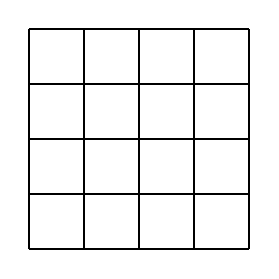
\begin{tikzpicture}[scale=0.7]
    \draw[step=1cm, black, thick] (0,0) grid (4,4);
\end{tikzpicture}
\\
Začetno stanje
\end{tabular}
&
\begin{tabular}{c}
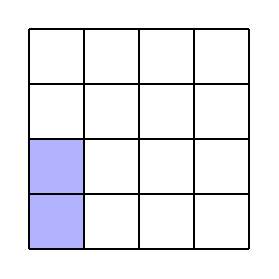
\begin{tikzpicture}[scale=0.7]
    \fill[blue!30] (0,0) rectangle (1,2);
    \draw[step=1cm, black, thick] (0,0) grid (4,4);
\end{tikzpicture}
\\
1. poteza
\end{tabular}
&
\begin{tabular}{c}
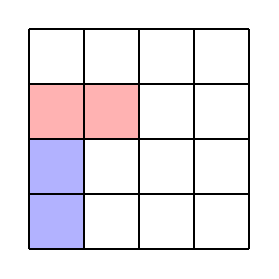
\begin{tikzpicture}[scale=0.7]
    \fill[blue!30] (0,0) rectangle (1,2);
    \fill[red!30] (0,2) rectangle (2,3);
    \draw[step=1cm, black, thick] (0,0) grid (4,4);
\end{tikzpicture}
\\
2. poteza
\end{tabular}
\\[1em]
\begin{tabular}{c}
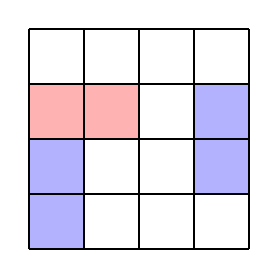
\begin{tikzpicture}[scale=0.7]
    \fill[blue!30] (0,0) rectangle (1,2);
    \fill[red!30] (0,2) rectangle (2,3);
    \fill[blue!30] (3,1) rectangle (4,3);
    \draw[step=1cm, black, thick] (0,0) grid (4,4);
\end{tikzpicture}
\\
3. poteza
\end{tabular}
&
\begin{tabular}{c}
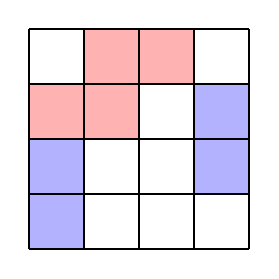
\begin{tikzpicture}[scale=0.7]
    \fill[blue!30] (0,0) rectangle (1,2);
    \fill[red!30] (0,2) rectangle (2,3);
    \fill[blue!30] (3,1) rectangle (4,3);
    \fill[red!30] (1,3) rectangle (3,4);
    \draw[step=1cm, black, thick] (0,0) grid (4,4);
\end{tikzpicture}
\\
4. poteza
\end{tabular}
&
\begin{tabular}{c}
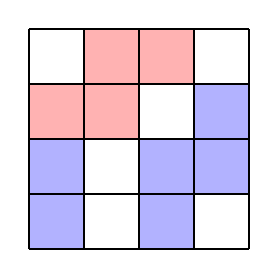
\begin{tikzpicture}[scale=0.7]
    \fill[blue!30] (0,0) rectangle (1,2);
    \fill[red!30] (0,2) rectangle (2,3);
    \fill[blue!30] (3,1) rectangle (4,3);
    \fill[red!30] (1,3) rectangle (3,4);
    \fill[blue!30] (2,0) rectangle (3,2);
    \draw[step=1cm, black, thick] (0,0) grid (4,4);
\end{tikzpicture}
\\
5. poteza
\end{tabular}
\\
\end{tabular}
\caption{Primer poteka igre (zmaga navpični igralec).}
\end{figure}

\section{Računska zahtevnost}
Za analizo računske zahtevnosti algoritmov uporabljamo asimptotično analizo, pri kateri uporabljamo veliko O notacijo. Ta opisuje, kako število operacij narašča glede na velikost vhodnih podatkov, pri čemer zanemarimo konstante in nižje redove. Kot primer lahko vzamemo algoritme za sortiranje. Za sortiranje tabele $N$ elementov bo algoritem, kot je quicksort, to opravil v $O(N \log N)$ operacijah, algoritem, kot bubble sort, pa v $O(N^2)$ operacijah.

V našem primeru želimo poiskati optimalno strategijo igre Domineering, za katero se izkaže, da asimptotična zahtevnost raste eksponentno. Natančneje jo lahko zapišemo kot $O(2^{W \cdot H})$, kjer $W$ in $H$ predstavljata širino in višino igralne plošče.

Do te predvidene asimptotične zahtevnosti pridemo na sledeč način. Predstavljajmo si igralno ploščo kot dvodimenzionalno tabelo. V tej bomo pisali ali je polje že zasedeno kot $True$ ali $False$ vrednost. Barva domine ki zaseda polje, nima vpliva na stanje. Optimalna poteza je torej odvisna le od zasedenosti posameznih polj in igralca, ki je na potezi. Ker je vsako polje lahko zapisano kot 0 ali 1, število možnih stanj narašča eksponentno in ga lahko opišemo s funkcijo $f(N) = 2^{N}$. V našem primeru je $N = W \times H$, kjer $W$ in $H$ predstavljata širino in višino igralne plošče. Ta analiza opisuje le zgornjo mejo števila stanj, saj niso nujno vsa stanja dosegljiva.

% Source - https://stackoverflow.com/a/73951765
% Posted by Celdor
% Retrieved 2026-03-24, License - CC BY-SA 4.0

\pgfplotsset{width=12cm,compat=1.18}
\begin{figure}[H]
    \centering
    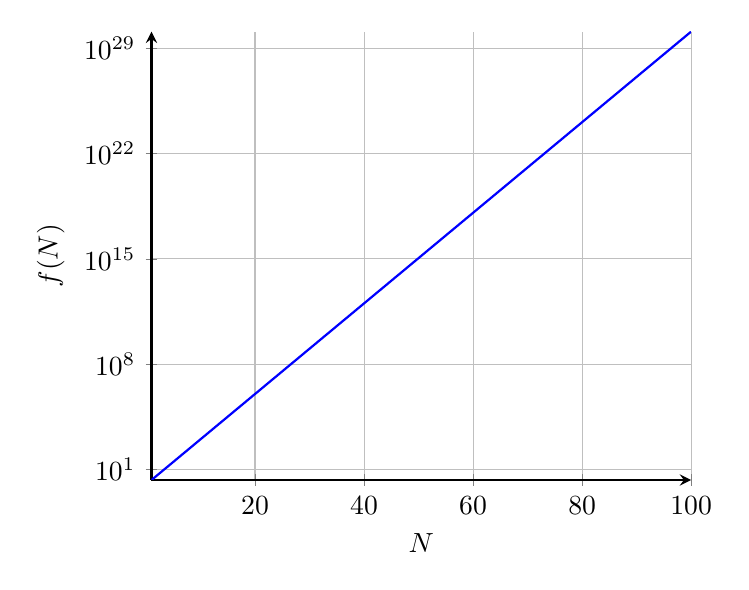
\begin{tikzpicture}
    \begin{axis}[
      axis lines=left,
      xmin=1, xmax=100,
      ymode=log,
      domain=0:100,
      samples=100,
      no markers,
      thick,
      grid=both,
      xlabel={$N$},
      ylabel={$f(N)$},
    ]
      \addplot+ {pow(2,x)};
    \end{axis}
    \end{tikzpicture}
    \caption{Prikaz $f(N)=2^N$ v logaritemski skali.}
    \label{fig:time_complexity_plot}
\end{figure}

\chapter{Algoritem za reševanje}
\section{Problem kot preiskovanje stanj}
Problem lahko predstavimo kot graf, kjer vsako vozlišče predstavlja možno stanje igralne plošče, povezave med vozlišči pa predstavljajo prehode med stanji oziroma odigrane poteze posameznega igralca. Pridobljen graf spada v družino dreves, ker ne vsebuje ciklov. To pomeni, da se iz nekega stanja ne moremo vrniti v že obiskano stanje. Takemu drevesu pravimo drevo igre (angl. \textit{game tree}). 

Ker smo že prej ugotovili, da naslednja poteza ni odvisna od preteklih potez, temveč le od trenutnega stanja plošče, lahko vsa vozlišča, ki predstavljajo enako stanje plošče združimo v eno vozlišče. Po izvedeni pretvorbi dobimo iz drevesa usmerjen acikličen graf. Takšna predstavitev omogoča učinkovitejše reševanje problema, saj se izognemo ponovni obravnavi enakih stanj.

Na sliki \ref{fig:3x3_game_graph} je prikazan primer grafa igre za $3 \times 3$ igralno ploščo. Barve vozlišč predstavljajo različna stanja: modra vozlišča predstavljajo zmagovalna stanja za prvega igralca, rdeča vozlišča predstavljajo zmagovalna stanja za drugega igralca, siva vozlišča pa predstavljajo stanja, ki jim algoritem še ni določil vrednosti.

\begin{figure}[H]
    \centering
    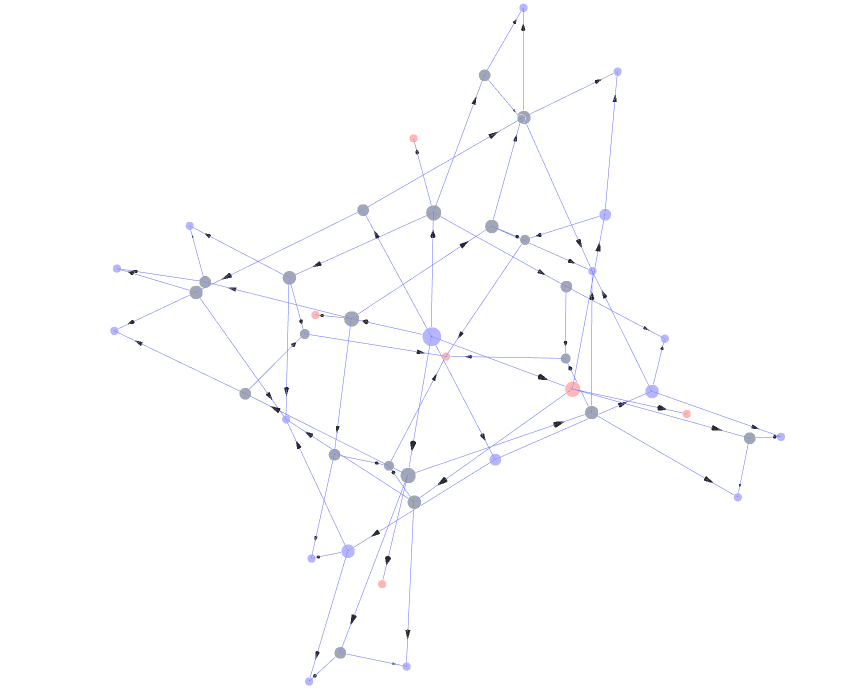
\includegraphics[width=0.75\linewidth]{images/3x3_game_graph.png}
    \caption{Primer grafa igre za $3 \times 3$ igralno ploščo.}
    \label{fig:3x3_game_graph}
\end{figure}

\section{Predstavitev igralnega stanja}
Dobljena stanja moramo tudi učinkovito shranjevati. Najbolj naravna ideja je hraniti dvodimenzionalno tabelo dimenzij $N \times M$ logičnih (bool) vrednosti. Pri tem za vsako stanje porabimo $N \times M$ bajtov. To je pri hranjenju velikega števila stanj zelo potratno in neučinkovito. Prvi korak pri izboljšavi tega pristopa je pretvorba dvodimenzionalne tabele v enodimenzionalno. Tako bomo do vrednosti na koordinatih $i$ in $j$ dostopali namesto z $A_{i,j}$, na način $A_{i\cdot M+j}$, kjer $A$ predstavlja tabelo igralne plošče.

Ker lahko hranimo le ali je polje zasedeno ali ne, lahko trenutno tabelo pretvorimo v zaporedje enic in ničel. To funkcionalnost pa lahko dosežemo že z najosnovnejšimi celoštevilskimi tipi, kot so 32, 64 in 128-bitna nepredznačena cela števila, in bitnimi operacijami za manipulacijo posameznih polj tabele. Takšna predstavitev bistveno zmanjša porabo pomnilnika in omogoča hitrejše izvajanje operacij nad stanji.

\section{Osnovni algoritem}
Algoritem je bil najprej zasnovan v najosnovnejši obliki. Uvrstimo ga lahko med brute force algoritme, saj preprosto preizkusi vse možne poteze, dokler ne najde zmagovalne strategije. Ker v teoretičnem najslabšem primeru obišče vsa veljavna izmed $O(2^{N \cdot M})$ možnih stanj, nekatera od teh pa celo večkrat, je hitrost reševanja že majhnih igralnih plošč slaba.

Tak algoritem deluje s pomočjo rekurzije. Recimo, da imamo rekurzivno funkcijo $search()$, ki kot parametra prejme trenutno stanje plošče in igralca, ki je trenutno na potezi. Na podlagi teh podatkov poskusi vse možne poteze in za vsako od njih rekurzivno nadaljuje iskanje s ponovnim klicem funkcije. Pri vsakem stanju algoritem preveri vse možne poteze in ugotovi, ali katera vodi v poraz nasprotnika. Če takšna poteza obstaja, jo algoritem izbere kot optimalno. Algoritem izvaja iskanje v globino po drevesu igre, kar ponazarja naslednja psevdokoda:

\begin{algorithm}[H]
\label{alg:basic_search}
\caption{Psevdokoda osnovnega algoritma}
\begin{algorithmic}[1]
\Function{Search}{state, turn}
    \If{ni možnih potez}
        \State \Return izguba
    \EndIf
    \For{vsaka možna poteza}
        \State next\_state $\gets$ izvedi potezo
        \If{\Call{Search}{next\_state, turn $\oplus$ 1} = izguba}
            \State \Return zmaga
        \EndIf
    \EndFor
    \State \Return izguba
\EndFunction
\end{algorithmic}
\end{algorithm}

\chapter{Optimizacije}
\section{Minimax}
Minimax je algoritem uporabljen za iskanje optimalne poteze na področju teorije iger, če predpostavimo, da nasprotnik igra optimalno. Algoritem in njegove variacije se pogosto uporabljajo tudi pri iskanju optimalnih strategij drugih iger za dva igralca, kot so tri v vrsto, backgammon in šah. Algoritem temelji na ideji, da je en igralec maksimizer, drugi pa minimizer. Maksimizer poskuša doseči čim višjo vrednost, minimizer pa čim nižjo vrednost. Vsakemu stanju plošče bomo dodelili vrednost, ki bo ali pozitivna, če je ugodno za maksimizerja, ali negativna, če je ugodno za minimizerja. 

Ko algoritem obravnava določeno stanje na drevesu, bo preveril, ali ima igralec na potezi, ki je trenutno na potezi možnost izbire poteze, ki vodi v stanje z ugodno vrednostjo. Če ne obstaja taka poteza, bomo trenutnemu stanju dodelili vrednost nasprotnega igralca. Primer tega je, če je na potezi maksimizer in ena poteza prinese vrednost $+1$, ostale pa vrednost $-1$. Ker ima vsaj eno možnost, bo tudi trenutno stanje označeno s $+1$.

Če ponovno pogledamo osnovni algoritem, bomo opazili, da je ideja minimax pristopa že uporabljena implicitno. To drži, saj osnovni algoritem že vrača dve različni vrednosti, kjer ena predstavlja zmago maksimizerja ($+1$), druga pa zmago minimizerja ($-1$).

\section{Memoizacija}
Memoizacija je tehnika hranjenja vrnjenih vrednosti funkcij, in priklic teh, namesto ponovnega računanja, ko bi bile te naslednjič potrebne. Sodi v širšo družino optimizacij, znanih kot dinamično programiranje. 

V našem primeru bo ta optimizacija zagotovila, da bo vsako stanje obiskano največ enkrat, a bomo za to potrebovali tudi podatkovno strukturo za hranjenje teh vrednosti. Ta optimizacija se pogosto uporablja pri rekurzivnih funkcijah, saj je nesmiselno večkrat računati isti podatek. Spodaj je podan diagram rekurzivnega računanja Fibonaccijevih števil.

\begin{figure}[H]
\centering
\forestset{
  called/.style={font=\bfseries},
  repeated/.style={
    text=gray,
    edge={->, draw=gray}
  }
}
\begin{forest}
for tree={edge={->}, minimum size=3mm, s sep=5mm, l=5mm}
[fib(6), called
  [fib(5), called
    [fib(4), called
      [fib(3), called
        [fib(2), called[1, called]]
        [fib(1), called[1, called]]
      ]
      [fib(2), repeated
        [1, repeated]
      ]
    ]
    [fib(3), repeated
      [fib(2), repeated [1, repeated]]
      [fib(1), repeated [1, repeated]]
    ]
  ]
  [fib(4), repeated
    [fib(3), repeated
      [fib(2), repeated [1, repeated]]
      [fib(1), repeated [1, repeated]]
    ]
    [fib(2), repeated [1, repeated]]
  ]
]
\end{forest}
\caption{Drevo klicev rekurzivne funkcije $fibonacci(6)$. Odvečni klici funkcije so pobarvani sivo.}
\end{figure}

\subsection*{Implementacija}
Za implementacijo memoizacije je bilo potrebno poiskati pravo podatkovno strukturo. Od te zahtevamo hiter dostop do vrednosti, možnost zapisa mnogih podatkov in možnost uporabe števila, ki predstavlja stanje, kot indeks. Tem zahtevam v C++ zadošča std::unordered\_map. Da osnovno verzijo algoritma dopolnimo, je potrebno le shranjevati vrnjene vrednosti funkcije in jih nato vračati, če so bile že izračunane.

\begin{algorithm}[H]
\label{alg:memo_search}
\caption{Psevdokoda algoritma z memoizacijo}
\begin{algorithmic}[1]
\State \textbf{unordered\_map} memo
\Function{Search}{state, turn}
    \If{state $\in$ memo}
        \State \Return memo[state]
    \EndIf
    \If{ni možnih potez}
        \State memo[state] $\gets$ izguba
        \State \Return izguba
    \EndIf
    \For{vsaka možna poteza}
        \State next\_state $\gets$ izvedi potezo
        \If{\Call{Search}{next\_state, turn $\oplus$ 1} = izguba}
            \State memo[state] $\gets$ zmaga
            \State \Return zmaga
        \EndIf
    \EndFor
    \State memo[state] $\gets$ izguba
    \State \Return izguba
\EndFunction
\end{algorithmic}
\end{algorithm}

\section{Bitne operacije}
Do te točke je bil eden najpočasnejših delov iskanja generacija naslednjih potez. To je potekalo z iteracijo čez vseh $W\cdot H$ možnih polj, tudi če so ta predstavljala neveljavne poteze. Da smo to pospešili, smo uporabili bitne operacije, saj z določenim zaporedjem operacij lahko dobimo masko vseh veljavnih potez v času $O(1)$ namesto v $O(N \cdot M)$. Ko imamo masko možnih potez, lahko uporabimo vgrajeno funkcijo, ki nam vrne število zaporednih ničel na koncu binarne predstavitve števila, iz česar lahko enolično določimo katero pozicijo domine bit predstavlja. 

\subsection*{Navpične poteze}
Za pridobitev bitne maske začetnih položajev, ko je na potezi navpični igralec, uporabimo naslednjo kombinacijo bitnih operacij, kjer spremenljivka $anchors$ prestavlja bitno masko izhodiščnih polj domin, $empty$ pa predstavlja bitno masko trenutno prostih polj. Vsak nastavljen bit v maski $anchors$ predstavlja začetni položaj možne poteze.

\[anchors = empty \land (empty\gg W)\]

\begin{figure}[H]
\centering
\begin{tabular}{ccc}
\begin{tabular}{c}
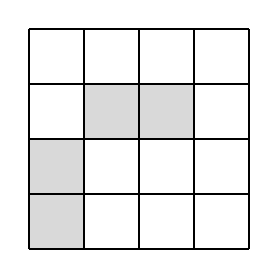
\begin{tikzpicture}[scale=0.7]
    \fill[gray!30] (0,0) rectangle (1,2);
    \fill[gray!30] (1,2) rectangle (3,3);
    \draw[step=1cm, black, thick] (0,0) grid (4,4);
\end{tikzpicture}
\\
$empty$
\end{tabular}
\begin{tabular}{c}
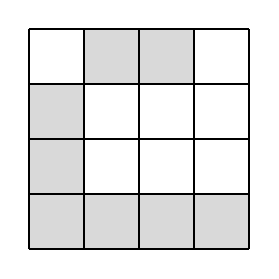
\begin{tikzpicture}[scale=0.7]
    \fill[gray!30] (0,1) rectangle (1,3);
    \fill[gray!30] (1,3) rectangle (3,4);
    \fill[gray!30] (0,0) rectangle (4,1);
    \draw[step=1cm, black, thick] (0,0) grid (4,4);
\end{tikzpicture}
\\
$empty \gg W$
\end{tabular}
\begin{tabular}{c}
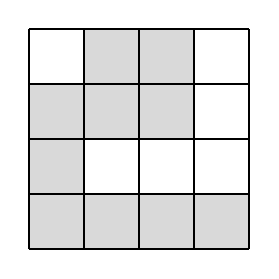
\begin{tikzpicture}[scale=0.7]
    \fill[gray!30] (0,0) rectangle (1,2);
    \fill[gray!30] (1,2) rectangle (3,3);
    \fill[gray!30] (0,1) rectangle (1,3);
    \fill[gray!30] (1,3) rectangle (3,4);
    \fill[gray!30] (0,0) rectangle (4,1);
    \draw[step=1cm, black, thick] (0,0) grid (4,4);
\end{tikzpicture}
\\
$anchors$
\end{tabular}
\\
\end{tabular}
\caption{Iskanje navpičnih potez z bitnimi operacijami. (Siva polja predstavljajo bitne $0$, bela polja pa bitne $1$.)}\end{figure}

\subsection*{Vodoravne poteze}
Podoben pristop bomo uporabili tudi pri iskanju bitne maske možnih potez za vodoravnega igralca. Dodatno potrebujemo še masko, ki predstavlja zadnji stolpec, označeno z $last$.

\[anchors = empty \land \lnot last  \land (empty\gg 1)\]

\begin{figure}[H]
\centering
\begin{tabular}{ccc}
\begin{tabular}{c}
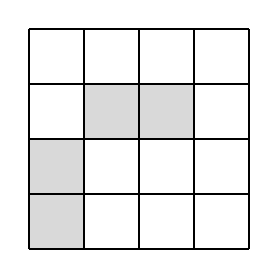
\begin{tikzpicture}[scale=0.7]
    \fill[gray!30] (0,0) rectangle (1,2);
    \fill[gray!30] (1,2) rectangle (3,3);
    \draw[step=1cm, black, thick] (0,0) grid (4,4);
\end{tikzpicture}
\\
$empty$
\end{tabular}
\begin{tabular}{c}
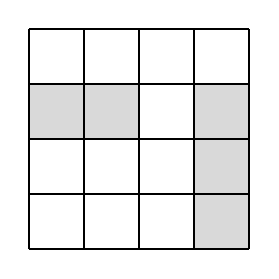
\begin{tikzpicture}[scale=0.7]
    \fill[gray!30] (0,2) rectangle (2,3);
    \fill[gray!30] (3,0) rectangle (4,3);
    \draw[step=1cm, black, thick] (0,0) grid (4,4);
\end{tikzpicture}
\\
$empty \gg 1$
\end{tabular}
\begin{tabular}{c}
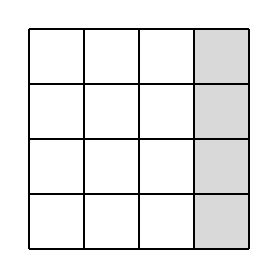
\begin{tikzpicture}[scale=0.7]
    \fill[gray!30] (3,0) rectangle (4,4);
    \draw[step=1cm, black, thick] (0,0) grid (4,4);
\end{tikzpicture}
\\
$\lnot last$
\end{tabular}
\begin{tabular}{c}
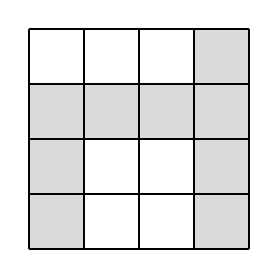
\begin{tikzpicture}[scale=0.7]
    \fill[gray!30] (0,0) rectangle (1,2);
    \fill[gray!30] (1,2) rectangle (3,3);
    \fill[gray!30] (0,2) rectangle (2,3);
    \fill[gray!30] (3,0) rectangle (4,3);
    \fill[gray!30] (3,0) rectangle (4,4);
    \draw[step=1cm, black, thick] (0,0) grid (4,4);
\end{tikzpicture}
\\
$anchors$
\end{tabular}
\\
\end{tabular}
\caption{Iskanje vodoravnih potez z bitnimi operacijami. (Siva polja predstavljajo bitne $0$, bela polja pa bitne $1$.)}
\end{figure}

Dobljeno množico možnih potez lahko dodatno optimiziramo tako, da jih ne obravnavamo v poljubnem vrstnem redu, temveč jih razvrstimo glede na verjetnost uspeha.

\section{Prioritizacija potez}
Prioritizacija potez spada v družino heurističnih optimizacij. Cilj teh je dodeliti možnim stanjem vrednosti, da jih lahko algoritem prioritizira in prej pregleda stanja, ki so ocenjena kot bližja optimalni rešitvi. V našem primeru bomo heuristično optimizirali izbiro prihodnjih potez. 

Do te točke smo preprosto iterirali čez vse poteze, urejene glede na njihov položaj na igralni plošči. Če pregledamo optimalne strategije, opazimo, da zelo pogosto postavljanje domin bližje sredini vodi do zmage. 

Da to dosežemo, bomo pred preizkušanjem različnih potez, vsaki potezi dodelili vrednost glede na oddaljenost izhodiščnega polja domine do sredine plošče, nato pa poteze razvrstili glede na pridobljene vrednosti. Nato bomo iterirali po sortiranem seznamu potez, kar v večini primerov vodi do hitrejšega izvajanja programa, saj se optimalna rešitev običajno najde prej. Kljub boljši učinkovitosti v praksi, ta pristop ne zagotavlja optimalnega vrstnega reda v vseh primerih. 

Vrednost poteze določimo kot razdaljo izhodiščnega polja domine do središča plošče:
\[
score = |i - i_c| + |j - j_c|
\]
kjer $(i, j)$ predstavlja koordinati izhodiščnega polja domine, $(i_c, j_c)$ pa središče plošče.

\section{Transpozicijska tabela}
Na tej točki z do sedaj omenjenimi optimizacijami naletimo na situacijo, ko čas izvajanja ni več glavni problem, temveč poraba pomnilnika zaradi uporabe podatkovne strukture std::unordered\_map v jeziku C++. Tudi če ta porablja le $O(S)$ pomnilnika, kjer $S$ predstavlja število shranjenih stanj, bo to pri večjih ploščah rastlo eksponentno.

Da se temu izognemo, potrebujemo podatkovno strukturo z omejeno velikostjo in s tem omejeno porabo pomnilnika. Izkaže se, da temu ustreza že preprosta enodimenzionalna tabela. Težava, ki se ponovno pojavi, pa je, kako bomo določali pozicije elementov v tabeli in kako ravnati v primeru, ko imamo več stanj kot prostora v tabeli. Oba problema lahko rešimo z razpršilno funkcijo, kombinaciji razpršilne funkcije in tabele pa pravimo transpozicijska tabela.

\subsection*{Obravnava trkov}
Pri uporabi transpozicijske tabele lahko pride do trkov, ko več različnih stanj preslikamo na isto mesto v tabeli. V takih primerih je potrebno določiti pravilo, katero vrednost obdržimo.

V naši implementaciji smo uporabili preprosto strategijo prepisovanja, kjer novo stanje vedno nadomesti obstoječe. Dadatno smo poskusili tudi strategiji, kjer dobi prioriteto stanje z večimi dominami. Pogosto se pri obravnavi iger uporablja kombinacija večih transpozicijskih tabel.

\section{Zobrist razprševalna funkcija}
Razpršilna funkcija je funkcija, ki preslika podatek v celo število, ki ga lahko uporabimo kot indeks v tabeli. Pri tem želimo, da so rezultati čim bolj enakomerno razporejeni, saj tako zmanjšamo število trkov.

V primeru iger se najpogosteje uporablja Zobristova razprševalna funkcija. Ta vsakemu polju na plošči dodeli naključno vrednost ob svoji inicializaciji. Da dobimo vrednost funkcije za neko stanje igre, bomo vzeli bitni XOR ($\oplus$) vseh vrednosti, ki pripadajo zasedenim poljem. Ker lahko operacijo XOR izvajamo inkrementalno, lahko vrednost funkcije posodobimo v času $O(1)$. Izkaže se, da so zaradi naključno dodeljenih vrednosti rezultati funkcije enakomerno razporejeni. 

Spodaj je podan primer inkrementalnega posodabljanja vrednosti funkcije, kjer $z_i$ predstavlja naključno vrednost, dodeljeno $i$-temu polju.

\begin{figure}[H]
\centering
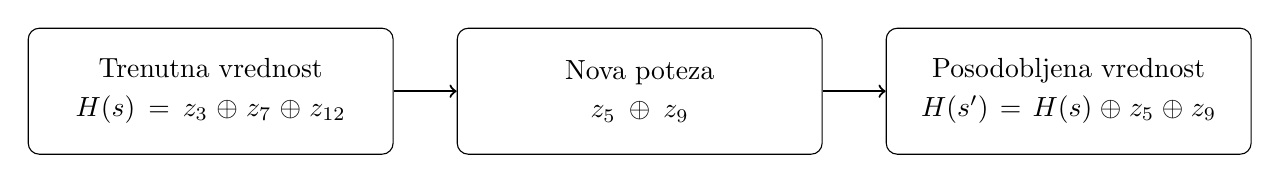
\begin{tikzpicture}[
    box/.style={
        draw,
        rounded corners,
        align=center,
        minimum height=1.6cm,
        text width=4.4cm
    },
    arrow/.style={->, thick}
]

\node[box] (old) {Trenutna vrednost\\[2pt] $H(s)=z_3 \oplus z_7 \oplus z_{12}$};
\node[box, right=8mm of old] (move) {Nova poteza\\[2pt] $z_5 \oplus z_9$};
\node[box, right=8mm of move] (new) {Posodobljena vrednost\\[2pt] $H(s') = H(s) \oplus z_5 \oplus z_9$};

\draw[arrow] (old) -- (move);
\draw[arrow] (move) -- (new);
\end{tikzpicture}
\caption{Inkrementalno posodabljanje Zobristove razprševalne vrednosti.}
\end{figure}

\section{Korenska paralelizacija}
Korenska paralelizacija je pristop, pri katerem paraleliziramo iskanje že pri prvi potezi oziroma na korenu drevesa igre. Namesto da vse možne začetne poteze obravnavamo zaporedno, vsako potezo obdelamo na ločeni niti. Ker so poddrevesa, ki izhajajo iz različnih začetnih potez, med seboj neodvisna, njihova vzporedna obravnava ne vplivna na pravilnost rezultata.

V implementaciji smo za vsako možno začetno potezo ustvarili ločeno nit, ki je izvajala iskanje optimalne strategije za pripadajoče poddrevo. Po najdenem zmagovalnem poddrevesu ali po obravnavi vseh poddreves se pridobljeni rezultati združijo in tako določijo optimalno potezo.

Ta pristop omogoča bistveno večji izkoristek pri večjedrnih procesorjih in lahko bistveno zmanjša čas izvajanja algoritma. To je še posebej učinkovit pristop pri uporabi na zmogljivejših sistemih kot so večjederni procesorji ali superračunalniki.

\chapter{Rezultati in analiza}
V tem poglavju analiziramo učinkovitost implementiranih algoritmov ter vpliv posameznih optimizacij. Za vsako različico algoritma bomo izmerili čas, porabljen pri iskanju strategije in obrazložili razloge za temi rezultati. Testiranje bo potekalo na prenosnem računalniku z AMD Ryzen 9 5900HX procesorjem z 8 jedri in 16GB rama, ter na Arnesovem superračunalniku z AMD EPYC 9254 procesorjem s 24 jedri in 128GB rama. Korenska paralelizacija je bila testirana na superračunalniku z 12 nitimi.

\section{Rezultati in analiza meritve časa}
Velika večina optimiziranih algoritmov, je rešila plošče do določene velikosti, pri večjih pa so algoritmi spodleteli saj bi porabili preveč časa za reševanje. Kljub temu je možno iz grafa razbrati nekaj anomalij in posebnosti. Na tem je prikazan porabljen čas pri iskanju rešitve, podatki pa so predstavljeni z logaritemsko skalo zaradi lažjega prikaza.
\definecolor{c1}{RGB}{227,119,194}  % pink
\definecolor{c2}{RGB}{140,86,75}    % brown
\definecolor{c3}{RGB}{44,160,44}    % green
\definecolor{c4}{RGB}{255,127,14}   % orange
\definecolor{c5}{RGB}{148,103,189}  % purple
\definecolor{c6}{RGB}{214,39,40}    % red
\definecolor{c7}{RGB}{31,119,180}   % blue

\begin{figure}[H]
\centering
\begin{tikzpicture}
\begin{axis}[
    width=15.5cm,
    height=10cm,
    xlabel={Velikost plošče},
    ylabel={Čas (ms)},
    ymode=log,
    grid=major,
    legend pos=north west,
    legend style={
        font=\footnotesize
    },
    tick label style={font=\small},
    label style={font=\small},
    xtick={16,20,25,30,36,42,49},
    xticklabels={4×4,4x5,5×5,5x6,6×6,6x7,7x7},
    every axis plot/.append style={thick},
    no markers,
    legend style={
        font=\footnotesize,
        at={(0.5,-0.18)},
        anchor=north,
        legend columns=4,
        column sep=15pt,
        draw=none
    }
]

\addplot[color=c1] table[x=size,y=bf,col sep=comma] {data/time.csv};
\addlegendentry{Osnovni}

\addplot[color=c2] table[x=size,y=memo,col sep=comma] {data/time.csv};
\addlegendentry{Memo}

\addplot[color=c3] table[x=size,y=bit,col sep=comma] {data/time.csv};
\addlegendentry{Bitne operacije}

\addplot[color=c4] table[x=size,y=mo,col sep=comma] {data/time.csv};
\addlegendentry{Prioritizacija}

\addplot[color=c5] table[x=size,y=bbmo,col sep=comma] {data/time.csv};
\addlegendentry{Bit. + Prior.}

\addplot[color=c6] table[x=size,y=ttmo,col sep=comma] {data/time.csv};
\addlegendentry{TT}

\addplot[color=c7] table[x=size,y=sup,col sep=comma] {data/time.csv};
\addlegendentry{Superrač.}

\end{axis}
\end{tikzpicture}
\caption{Primerjava časa izvajanja različnih optimizacij.}
\end{figure}

\subsection{Bitne operacije in prioritizacija}
Pri treh rešitvah (prioritizacija, bitne operacije in kombinacija teh dveh) je možno opaziti, da se ustavijo na isti točki pri $6 \times 6$ ploščah. Razlog za to ni pomanjkanje hitrosti algoritmov, temveč velika poraba pomnilnika zaradi shranjevanja obiskanih stanj. Ko program prekorači to točko, vse operacije postanejo drastično počasnejše in s tem prepočasne, da bi program lahko v sprejemljivem času končal izvajanje. To kaže, da je poraba pomnilnika v praksi enako pomembna omejitev kot časovna zahtevnost algoritma.

\subsection{Transpozicijska tabela}
Pri algoritmih, ki uporabljajo transpozicijsko tabelo, so časi izvajanja pri manjših ploščah skoraj konstantni. Razlog za to je, da se velika količina pomnilnika za tabelo alocira že na začetku izvajanja, kar predstavlja glavni del časa izvajanja pri manjših problemih. Prav tako zaradi kolizij izgubimo na hitrosti izvajanja, a je to problem, ki se mu ne moremo izogniti zaradi velikosti igralnih plošč.

\subsection{Superračunalnik}
Optimizacija s paralelizacijo je bila uporabljena samo na superračunalniku. Razlog za to je pomanjkanje pomnilnika na osebnem računalniku, saj se pri preiskovanju vsakega od poddreves uporablja svoja transpozicijska tabela. Kljub temu da razlika na grafu zaradi logaritmične skale ni izrazita, uporaba paralelizacije čas izvajanja približno prepolovi. To potrjuje, da je korenska paralelizacija učinkovita predvsem pri večjih problemih, kjer je mogoče izkoristiti več procesorskih jeder.

\section{Povzetek analize}
Na splošno rezultati kažejo, da posamezne optimizacije bistveno izboljšajo učinkovitost algoritma. Največji vpliv je imela memoizacija, ki bistveno zmanjša število obdelanih stanj, medtem ko bitne operacije in prioritizacija izboljšajo hitrost izvedbe posameznih korakov iskanja. Transpozicijska tabela omogoča obravnavo večjih problemov, kar z uporabo najivnih metod memoizacije ne bi bilo mogoče. Kljub optimizacijam problem ostaja eksponenten, kar pomeni, da velikost plošč, ki jih lahko obravnavamo, ostaja omejena.

\chapter{Zaključek}

V nalogi smo obravnavali problem iskanja optimalne strategije v igri Domineering in ga predstavili kot problem preiskovanja prostora stanj. Začeli smo z implementacijo osnovnega algoritma, ki z uporabo rekurzije preizkusi vse možne poteze, nato pa smo ga postopoma izboljševali z različnimi optimizacijami.

Kljub vsem optimizacijam problem ostaja zaradi eksponentne rasti prostora stanj računsko zahteven, kar nas tudi omejuje na manjše plošče, če želimo, da se program izvede v razumnem času. Pri večjih problemih se kot največja omejitev izkaže poraba pomnilnika.

Pri razvoju algoritma smo se srečali z več izzivi, predvsem pri iskanju novih optimizacij, ki bi bile smiselne pri reševanju našega problema. Kljub obstoju dodatnih optimizacij, ki bi lahko še izboljšale rezultate, se nanje nismo osredotočili, saj zahtevajo poglobljeno matematično znanje in teorijo iger.

Naloga tako pokaže, da lahko z uporabo pravilnih pristopov bistveno izboljšamo učinkovitost reševanja zastavljenega problema, vendar kljub temu temeljna računska zahtevnost omejuje možnost izboljšave. 

\begin{thebibliography}{9}

\bibitem{domineering-paper-counting}
S. Huntemann, N. A. McKay: \emph{Counting Domineering Positions}.  
Journal of Integer Sequences, Vol. 24 (2021).  
Dostopno na: \url{https://cs.uwaterloo.ca/journals/JIS/VOL24/Huntemann/hunt2.pdf}.

\bibitem{domineering-paper-8x8}
D. M. Breuker, J. W. H. M. Uiterwijk, H. J. van den Herik: \emph{Solving 8 $\times$ 8 Domineering}.  
Theoretical Computer Science 230 (2000).  
Dostopno na: \url{https://www.researchgate.net/publication/220149719_Solving_88_Domineering}.

\bibitem{domineering-paper-11x11}
J. W. H. M. Uiterwijk: \emph{11 $\times$ 11 Domineering is Solved: The first player wins}.  
Theoretical Computer Science.  
Dostopno na: \url{https://arxiv.org/abs/1602.05404}.

\bibitem{cp-algorithms}
CP-Algorithms: \emph{Game Theory}.  
Dostopno na: \url{https://cp-algorithms.com/}.

\bibitem{chess-programming-wiki}
Chess Programming Wiki: \emph{Zobrist Hashing}.  
Dostopno na: \url{https://www.chessprogramming.org/Zobrist_Hashing}.

\bibitem{al-go-rithms}
Z. Pandovski: \emph{al-go-rithms}.  
Dostopno na: \url{https://github.com/ZoranPandovski/al-go-rithms}.

\end{thebibliography}

\chapter*{Izjava o avtorstvu}

Izjavljam, da je strokovno poročilo Reševanje igre Domineering v celoti moje avtorsko delo, ki sem ga izdelal samostojno s pomočjo navedene literature in pod vodstvom mentorja.

\vspace{2cm}

\noindent
Ljubljana, \today \hfill Vid Furlan

\vspace{2cm}

\hfill\rule{6cm}{0.4pt}

\end{document}